              
\documentclass[fleqn,10pt]{wlscirep}
\title{Scientific Reports Title to see here (20 words or less)}
\author[1]{Rachel LeCover}
\author[1,*]{Jeffrey D. Varner}
\affil[1]{Affiliation, School of Chemical and Biomolecular Engineering, Ithaca NY, 14852, USA}
\affil[*]{jdv27@cornell.edu}
%\keywords{Keyword1, Keyword2, Keyword3}
\begin{abstract}
Example Abstract. Abstract must be under 200 words and not include subheadings or citations. Example Abstract. Abstract must be under 200 words and not include subheadings or citations. Example Abstract. Abstract must be under 200 words and not include subheadings or citations. Example Abstract. Abstract must be under 200 words and not include subheadings or citations. Example Abstract. Abstract must be under 200 words and not include subheadings or citations. Example Abstract. Abstract must be under 200 words and not include subheadings or citations. Example Abstract. Abstract must be under 200 words and not include subheadings or citations. Example Abstract. Abstract must be under 200 words and not include subheadings or citations. 
\end{abstract}
\begin{document}
\flushbottom
\maketitle
% * <john.hammersley@gmail.com> 2015-02-09T12:07:31.197Z:
%
%  Click the title above to edit the author information and abstract
%
\thispagestyle{empty}
\noindent Please note: Abbreviations should be introduced at the first mention in the main text – no abbreviations lists. Suggested structure of main text (not enforced) is provided below.
\section*{Introduction}
The rate at which a heart beats is determined, in part, by the sympathetic and parasympathetic portions of the nervous system. When the sympathetic nervous system is stimulated, it releases epinephrine and norepinephrine  which increase heart rate. The parasympathetic system releases acetylcholine which decreases heart rate.  These two systems, often described as an accelerator and a brake, are not totally independent on each other, rather, they interact through second messengers cAMP and cGMP. \cite{olshansky2008parasympathetic}
Heart rate is also controlled by the baroreflex system. The baroreflex system consists of baroreceptors, tension sensitive nerve endings found in the circulatory system. \cite{ottesen1997modelling} When they sense a change in pressure, they cause a change in the frequency of nerve activity. When pressure (and stretch) rapidly increase, so does the baroreceptor firing rate. \cite{negative1999reflexes} This effects of this signal are not instantaneous, rather, there is a time delay on the order of seconds before the sympathetic and parasympathetic nervous systems respond. \cite{ottesen1997modelling}

Olufsen and Ottesen have developed models of heart rate based on blood pressure measurements.\cite{olufsen2013practical} From the blood pressure measurement, the model predicts a firing rate for different types of receptors, which is then used to predict the response times of the parasympathetic and sympathetic nervous system. The response times are then used to predict dimensionless norepinephrine and acetylcholine concentrations, which are finally used to predict heart rate. 

We used the MIMIC II Waveform Database as the source of the pressure and heart rate data used to test this model.\cite{saeed2011multiparameter} MIMIC contains de-identified data from patients who visited the Beth Israel Deaconess Medical Center ICU. This database contains a wealth of information: diagnoses, demographics, clinical data, such as heart rate and intravenous medications as well as laboratory results.  
A subset of the MIMIC II Waveform Database has been linked to patients found in the MIMIC II Database, allowing us to combine the waveforms with demographic information. From this subset, we selected patients that had numerics records with data recorded once per second with more than five data points available in the first 10 minutes of recorded data, giving us 273 patients meeting this criteria.
To our knowledge, this is the first study to attempt to model heart rate as a function of blood pressure for such a large number of patients. Additionally, many previous studies were performed with healthy patients, in contrast, this study focuses on intensive care unit patients. 
\section*{Results}
\subsection*{One Dimensional Optimization of Parameters}
We minimized averaged the mean squared error per patient using the Nelder Mead algorithm as implemented in Julia package NLopt. We forced all of the parameters to be non-negative as to be biologically correct.The original and estimated values of the parameters are shown in Table \ref{tab:SingleParamsNLopt}. %The value of $\tau_2$ decreased dramatically in the estimated parameter set, increasing the effect of $n_1$ on the firing rate. Additionally, $\tau_{ach}$ increased significantly, reducing the changes in $c_{ach}$. As shown in Figure \ref{fig:paramscomparsion}, the estimated parameters tend to smooth out the varaibility in the predicted heart rate compared to the original parameters. The change in parameters reduced the mean squared error, averaged over all of the selected patients, from 1167 to 349.

Within the estimated parameter set, the value of $N$, the baseline firing rate increased, and both $k_1$ and $\tau_1$, representing a change in the response rate of the faster firing baroreceptors in the model. Baroreceptors are generally divided into three groups, depending on their transmission speeds (on the order of half a second, five seonds, and five hundred seconds), but this model only includes two types. \cite{ottesen1996non} The increase in $\tau_1$ and the decrease in $\tau_2$ in the estimated parameter set may be the result of oversimplification. 

The baseline heart rate ($h_0$) decreased slightly, to 88 bpm, from the initial 100 bpm. Both $\tau_{ach}$ and $m_{ach}$, which determine how acetylcholine plays into the model, decreased dramatically in the estimated parameter set, with the reduction in $m_{ach}$ reducing the effects of a change in acetylcholine on heart rate, and the decrease in $\tau_{ach}$ increasing the rate of acetylcholine change. The estimated parameter set reduced the averaged mean squared error to 352 from 1167. As seen in Figure \ref{fig:paramscomparsionNLopt}, the estimated parameters slightly overestimate heart rate for this patient, but they perform far better than the original parameters, which severely underestimate the heart rate. This behavior is typical of the model on patients in this study.

$k_1$ and $\beta$ were held constant as to reduce the search space. $\alpha$, the parameter used to smooth the pressure data was held constant at 1.5 to smooth the data with a minimal phase shift. The maximum firing rate, $M$, was held constant, as it only appears in this system of equations by normalizing $n$. The sympathetic nervous system delay, $\tau_d$, was held constant, owing to the propagation of discontinuities. \cite{baker1997pitfalls}


\subsection*{Clustering}
We clustered the patients based on their age, average heart rate, and SAPS (Simplified Acute Physiology) score, a measure that estimates a patient's risk of death within an intensive care unit.\cite{le1993new} We used the patient's average SAPS since some patients had multiple admissions resulting in more than one blood pressure-heart rate track. 
Through the use of the Clustering Julia package, we created up to 26 clusters based on these variables, and scored each cluster with the sum of its silhouettes, where a higher score means that each member of the cluster is more similar to the other members of the clusters.\cite{rousseeuw1987silhouettes} We found that grouping the patients into two clusters gave the highest score and therefore the best clustering. The sum of silhouettes as a function of number of clusters is shown in \ref{fig:sumofsils}, and the patients by cluster in \ref{fig:clusteredpatients}. Cluster 1 patients (n = 165), shown in white, tend to have a lower average heart rate (73 BPM compared to 88 BPM), and be older than patients in cluster 2 (n = 108) (69 years vs 59 years, on average). 
\subsection*{Multidimensional Optimization}
We used the Julia language POETs package, which combines simulated anealing with Pareto optimality to generate families of best parameters.\cite{bassen2016jupoets} Using the two clusters formed by k-means, we minimized the averaged mean squared error to create these parameter families. We utilized a monotonically decreasing cooling schedule with five iterations at each temperature. The trade off curve generated using $\alpha$ = .9 is shown in \ref{fig:tradeoffcurve}, and with $\alpha$ =.5  in \ref{fig:tradeoffcurveslower}. We used the parameter families from the slower cooling for further analysis. 
To decrease the time necessary to perform the simulated annealing, we utilized Julia's transparent parallelization capabilities. With the @parallel (+) operator, we were able to calculate patient's mean squarred errors in parallel. The speed up from parallelization is shown in \ref{fig:executiontime}. 
We then selected the ten best sets of parameters from each cluster to examine the performance of the model with the new parameters. A sample patient from cluster 1 is shown in \ref{fig:cluster1patientmulti}, and from cluster 2 in \ref{fig:cluster2patientmulti}. The new parameter families reduced the averaged mean squared error even further than the parameters estimated using Nelder Mead-the ten best families for cluster 1 reduced the averaged mean squared error to 135 or less, and for cluster two, the averaged mean squared error was reduced to 178, or less. 

Both of the families had fairly similar values for $m_{nor}$ and $m_{ach}$, however, cluster 1 had a larger value of $N$, the resting firing rate than cluster 2. Cluster 1 contains the older patients, on average, suggesting that the resting firing rate may be age dependent. The differences in average heart rate between the clusters apparent in the clustering are appearent in the difference in $h_0$ between the two clusters, with cluster 2 having a faster base line heart rate, at $1.749 \pm .05$ beats per second, corresponding to $104.95 \pm 3$ beats per minute, compared to $74.4 \pm 4$ beats per minute for cluster 1.
 
\subsection*{Sensitivity Using Finite Differences}
The derivatives of all parameters were estimated using central differences. 
\begin{equation}
\frac{dh}{d\theta_j} = \frac{h(\theta_0+\frac{e_j}{2})-h(\theta_0-\frac{e_j}{2})}{\delta}
\end{equation}
where $\delta=10^{-8}*\theta_j$ and $e_j$ is a vector of length $\delta$ in the $j^{th}$ direction.
To collapse the time dimension, we calculated overall state sensitivity coefficients. \cite{stelling2004robustness}
\begin{equation}
S_{0j}(t) = \frac{1}{n_s}p_j \left(\sum_{k=1}^{n_t} \sum_{i=1}^{n_s} \left[ \frac{1}{x_i} \frac{dx_i(t_k)}{dp_j} \right]^2 \right)^{1/2}
\end{equation}
where $n_s$ = 1, as $h$ is the only state variable and $n_t$ is the number of time points available for that patient. We calculated sensitivites of parameters that were optimized and not that of those held constant.
\subsubsection*{Single Objective Sensitivity}
From the original values provided by Olufsen and Ottesen, we found that $h_0$ was the most sensitive parameter, followed by $N$, $m_{ach}$, and $m_{nor}$ in that order. Of the four most sensitive equations, three of them ($h_0$, $m_{ach}$ and $m_{nor}$) appear directly in the equation for heart rate, and $N$ indirectly appears, as both $c_{ach}$ and $c_{nor}$ are functions of $N$.
The four parameters that were the most sensitive in our study were among the five most sensitive parameters found by Olufsen and Ottesen, as seen in \ref{tab:OSSCsoriginalParams}.
\subsubsection*{Multiobjective Sensitivity} 
For the multiobjective case, we used the same finite differences, but averaged them not only over the patients, but over the families of parameters-the ten best for each cluster. As with the single objective case, $h_0$ is the most sensitive parameter, followed by $N$, as seen in \ref{fig:MultiobjectiveSensitivityGraph}.
\section*{Discussion}
The Discussion should be succinct and must not contain subheadings.
\section*{Methods}
All calculations were carried out Ubunutu 16.04 using Julia version .0.4.5, with 7.7 GB of available RAM on a Intel Core i7-6700 CPU @ 3.40GHz. Differential equations were solved using the ODE package, with solvers ode23 and ode78, with an absolute and relative tolerance of $10^{-8}$. 
\bibliography{draft1}
\section*{Acknowledgements (not compulsory)}
Acknowledgements should be brief, and should not include thanks to anonymous referees and editors, or effusive comments. Grant or contribution numbers may be acknowledged.
\section*{Author contributions statement}
Must include all authors, identified by initials, for example:
A.A. conceived the experiment(s),  A.A. and B.A. conducted the experiment(s), C.A. and D.A. analysed the results.  All authors reviewed the manuscript. 
\section*{Additional information}
To include, in this order: \textbf{Accession codes} (where applicable); \textbf{Competing financial interests} (mandatory statement). 
The corresponding author is responsible for submitting a \href{http://www.nature.com/srep/policies/index.html#competing}{competing financial interests statement} on behalf of all authors of the paper. This statement must be included in the submitted article file.

%\begin{figure}[ht]
%                \centering
%        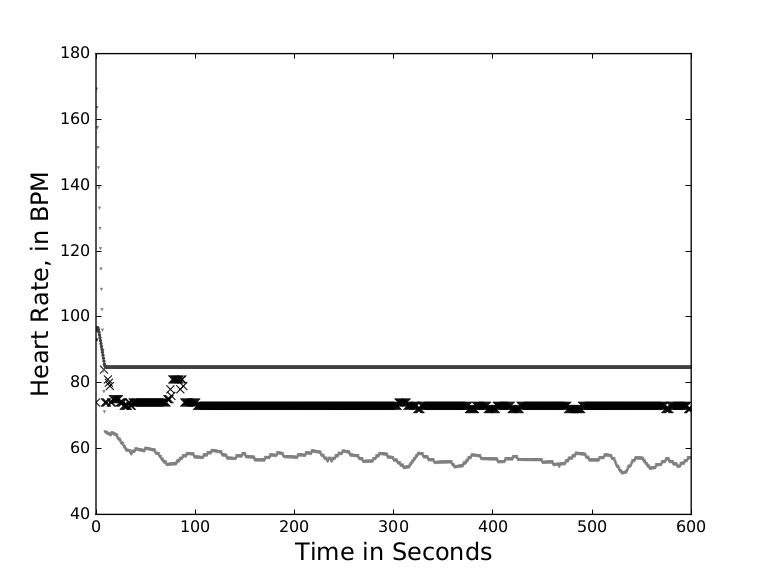
\includegraphics[width=\linewidth]{figures/paramscomparisons28611-3108-03-06-18-24n}
%       \caption{The black xs are the measured heart rate, the dark gray is the model prediction using the original parameters and the light gray is the model prediction using the original parameters.}
%       \label{fig:paramscomparsion}
%\end{figure}

\begin{figure}[ht]
                \centering
        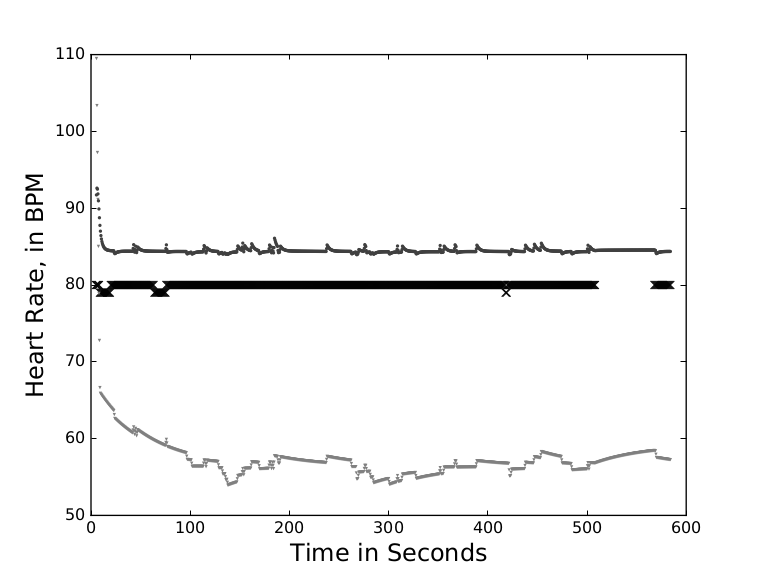
\includegraphics[width=\linewidth]{figures/s27193-3271-03-15-13-26n}
       \caption{The black xs are the measured heart rate, the dark gray is the model prediction using the original parameters and the light gray is the model prediction using the original parameters.}
       \label{fig:paramscomparsionNLopt}
\end{figure}


\begin{figure}[ht]
                \centering
        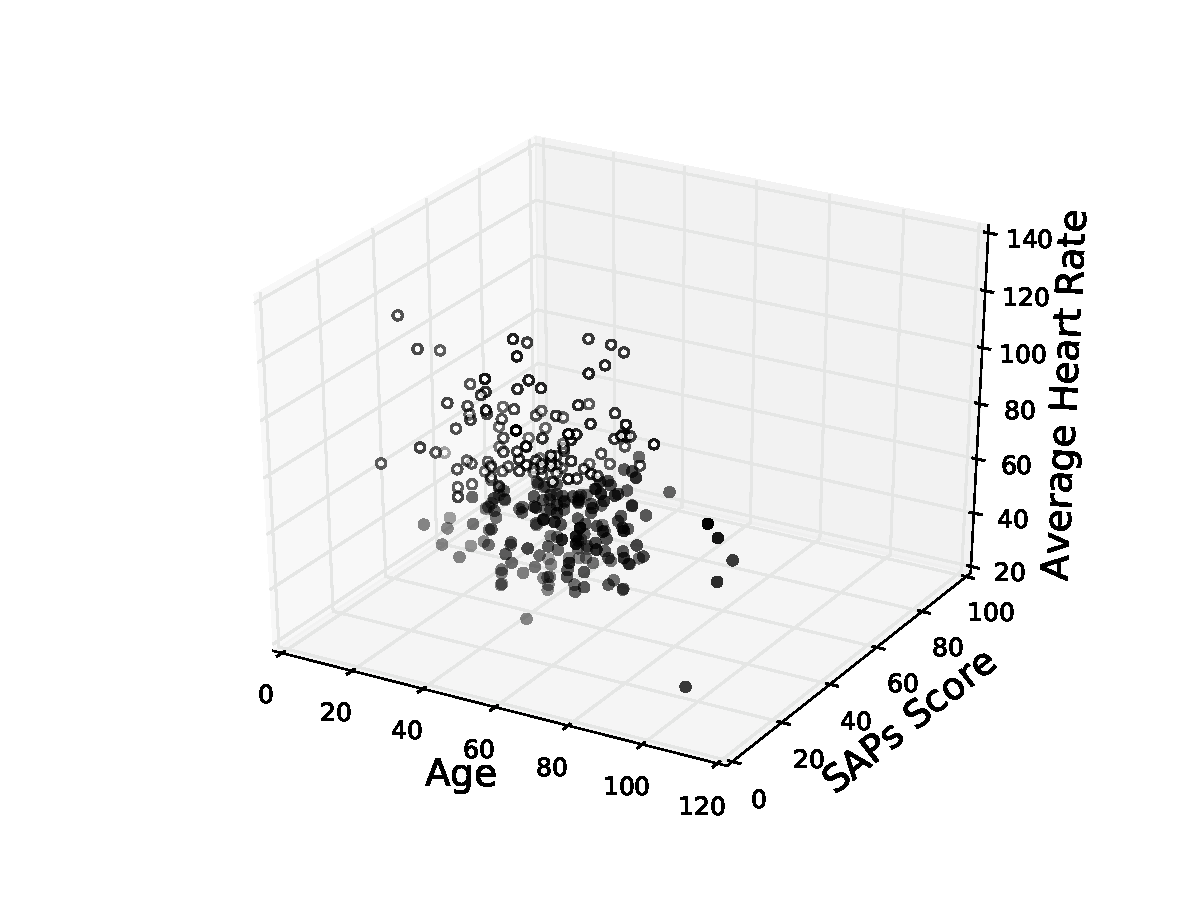
\includegraphics[width=\linewidth]{figures/2clusters}
       \caption{The patients, clustered into two groups.}
       \label{fig:clusteredpatients}
\end{figure}

\begin{figure}[ht]
                \centering
        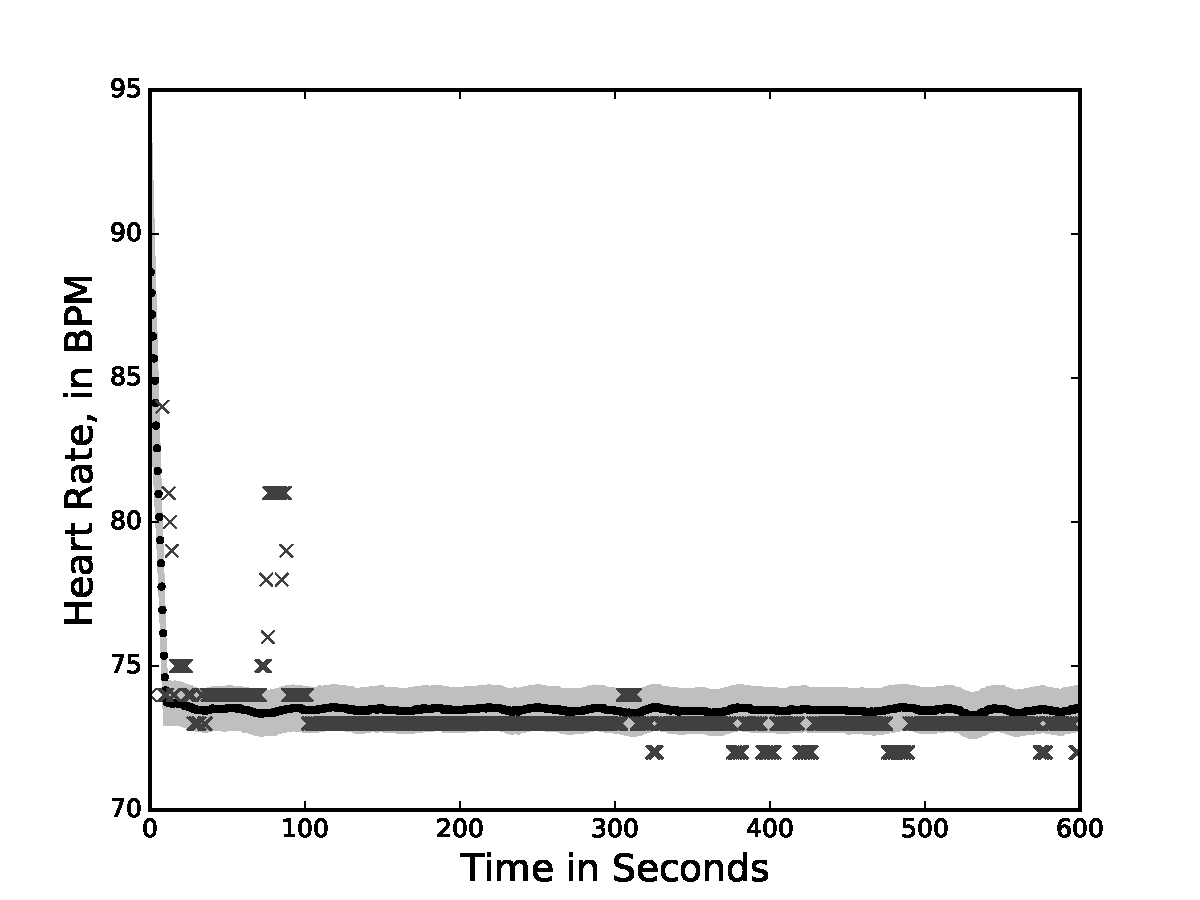
\includegraphics[width=\linewidth]{figures/timedatausingdifferentparamsetsforpatients28611-3018-03-06-18-24n}
       \caption{Performance of the model on a patient in cluster 1. The x represent the true heart rate, the black dots are the mean model prediction from the family of best parameter sets, and the grey gives a 95\% confidence interval.}
       \label{fig:cluster1patientmulti}
\end{figure}
\begin{figure}[ht]
                \centering
        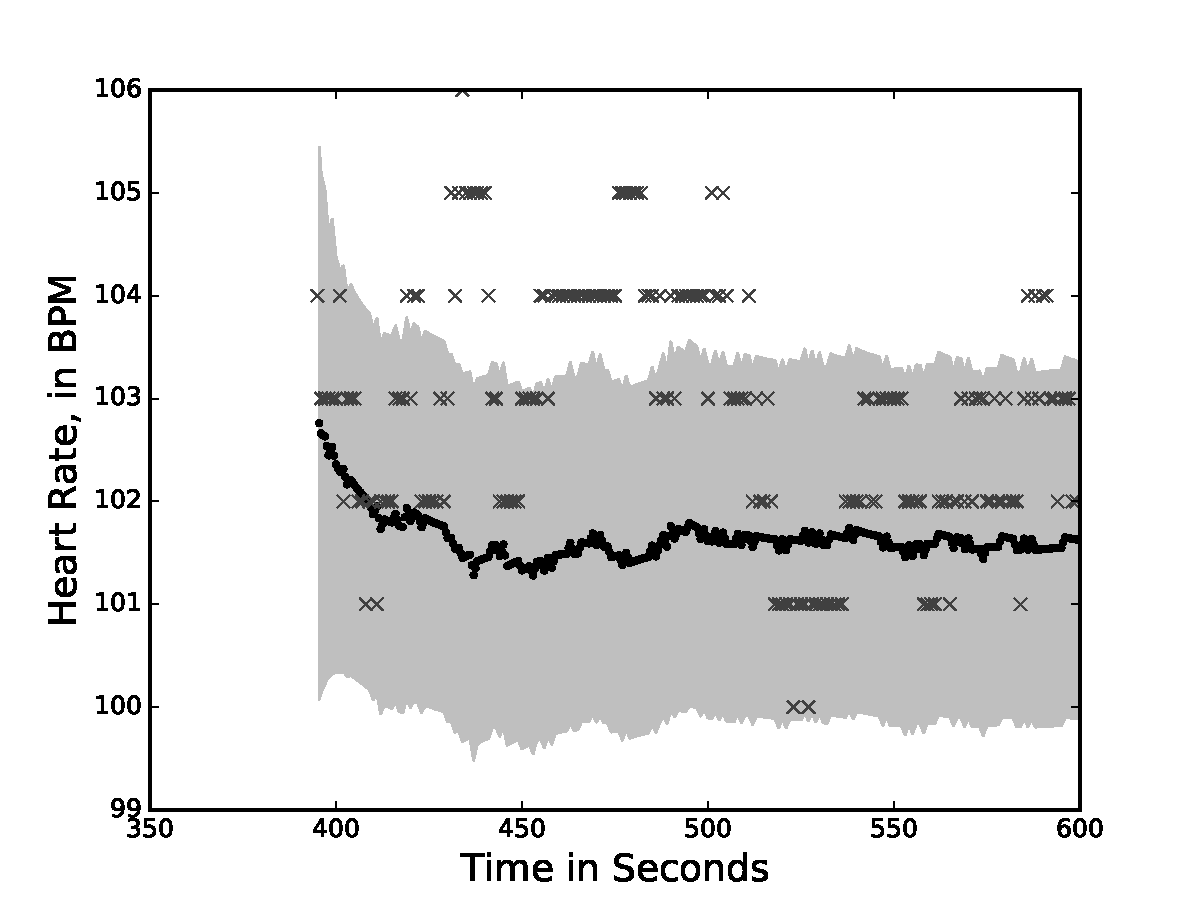
\includegraphics[width=\linewidth]{figures/timedatausingdifferentparamsetsforpatients32582-3106-02-22-22-22n}
       \caption{Performance of the model on a patient in cluster 2. The x represent the true heart rate, the black dots are the mean model prediction from the family of best parameter sets, and the grey gives a 95\% confidence interval.}
       \label{fig:cluster2patientmulti}
\end{figure}
\begin{figure}[ht]
                \centering
       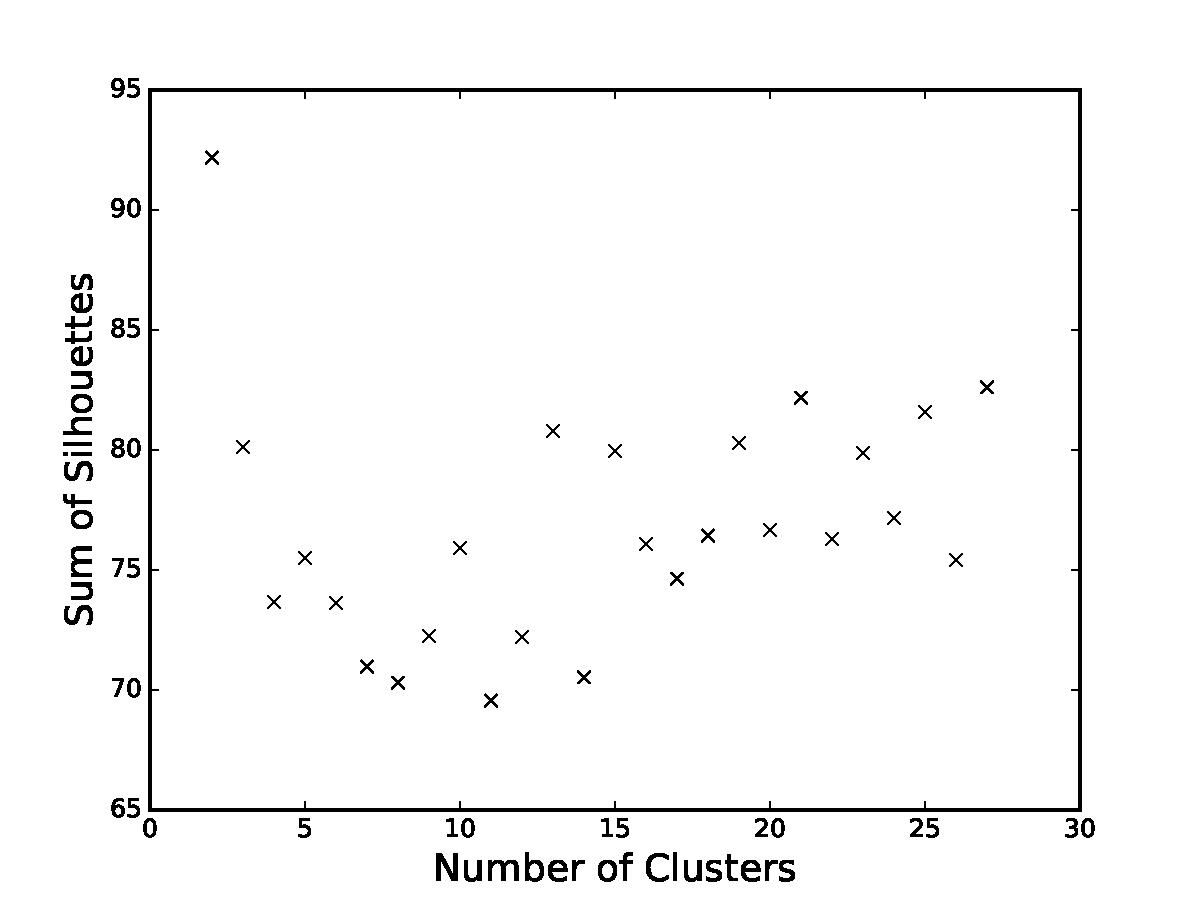
\includegraphics[width=\linewidth]{figures/sumofsilhouettesasafunctionofclustersjustAgeSAPSavgHR}
       \caption{Sum of silhouettes as function of number of clusters}
       \label{fig:sumofsils}
\end{figure}
\begin{figure}[ht]
       \centering
       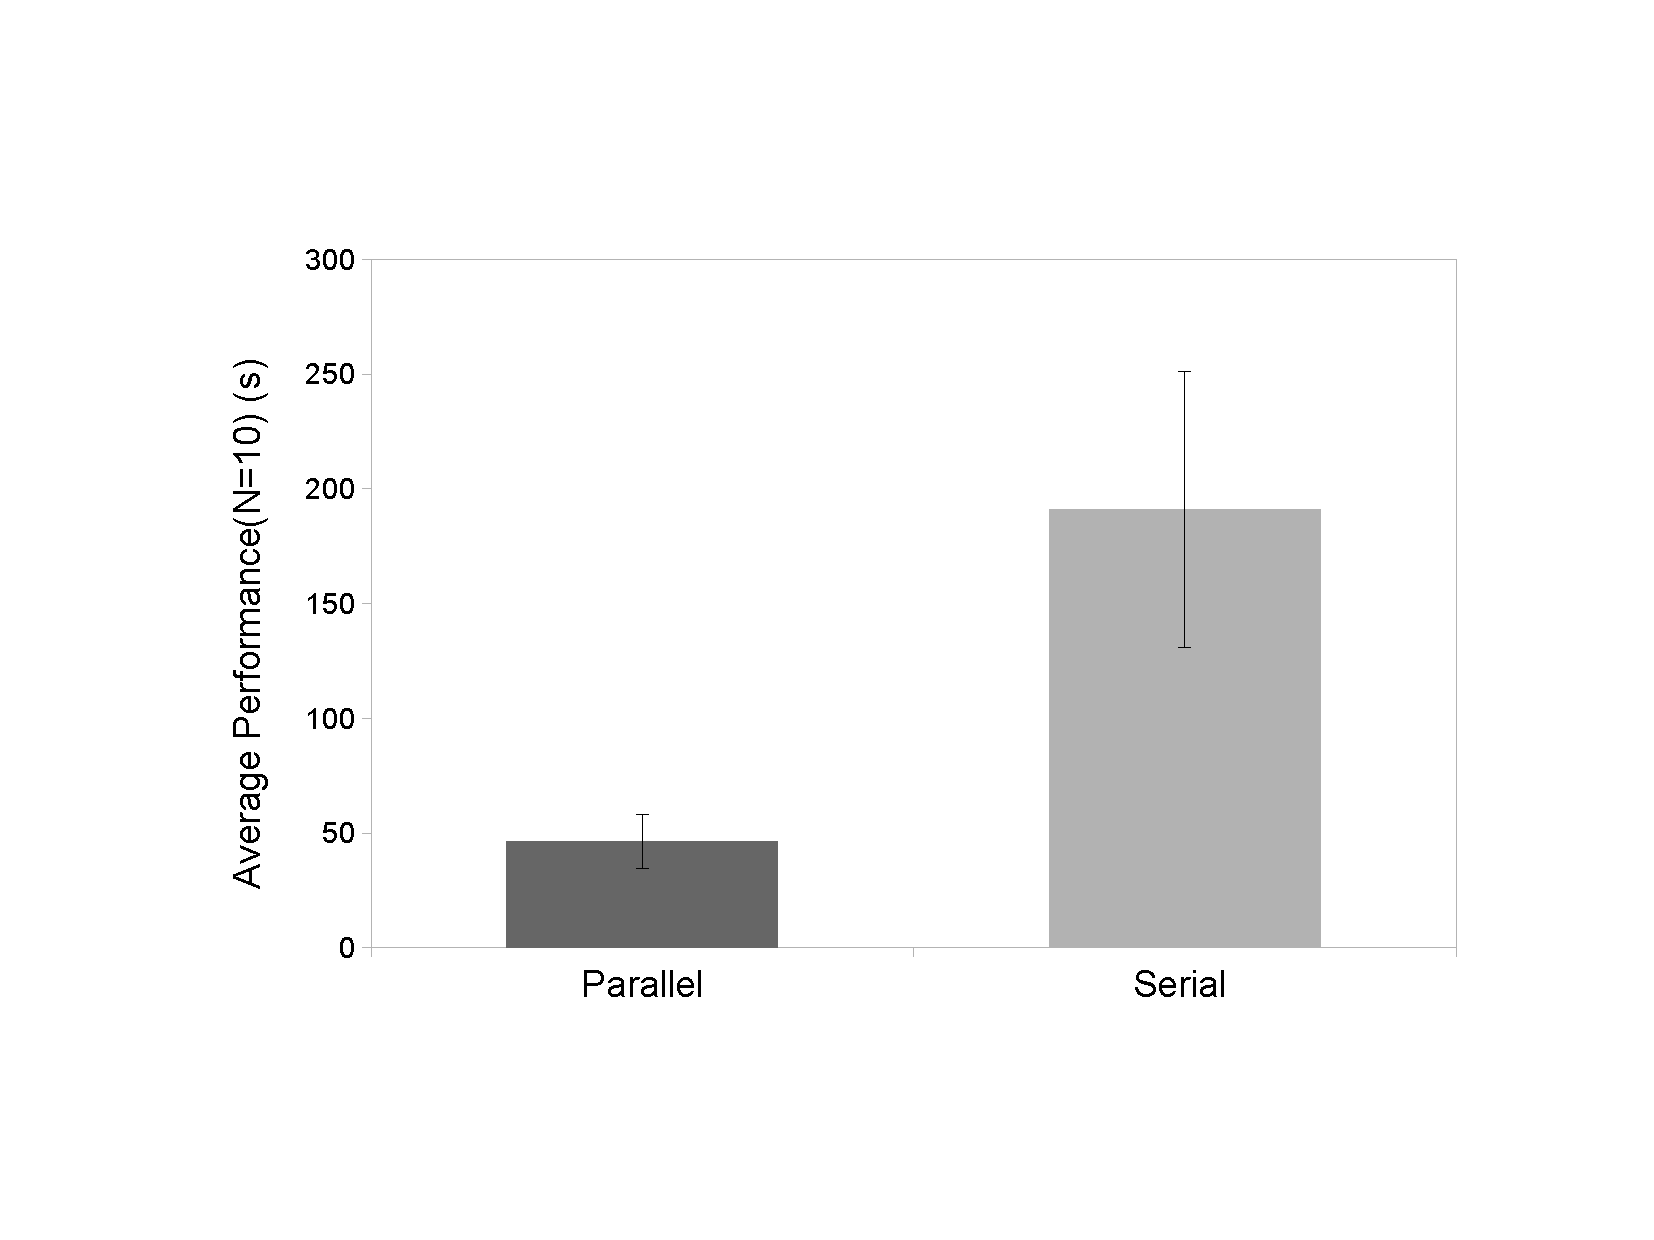
\includegraphics[width=\linewidth]{figures/runtimecomparison}
       \caption{Switching from serial to parallel computation resulted in a significant speed up. In parallel operation, six cores were used.}
        \label{fig:executiontime}
\end{figure}
\begin{figure}[ht]
       \centering
       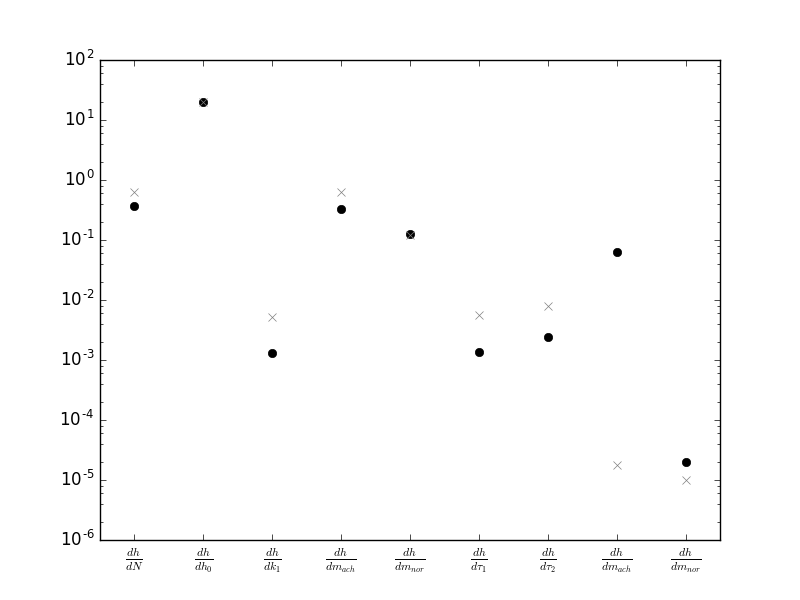
\includegraphics[width=\linewidth]{figures/MultiobjectiveSenstivityGraph10familiesofNoErrorBars}
       \caption{The black circles are from cluster 1, the grey x's represent cluster 2. Error bars are omitted for the sake of clarity.}
        \label{fig:MultiobjectiveSensitivityGraph}
\end{figure} 
\begin{figure}[ht]
       \centering
       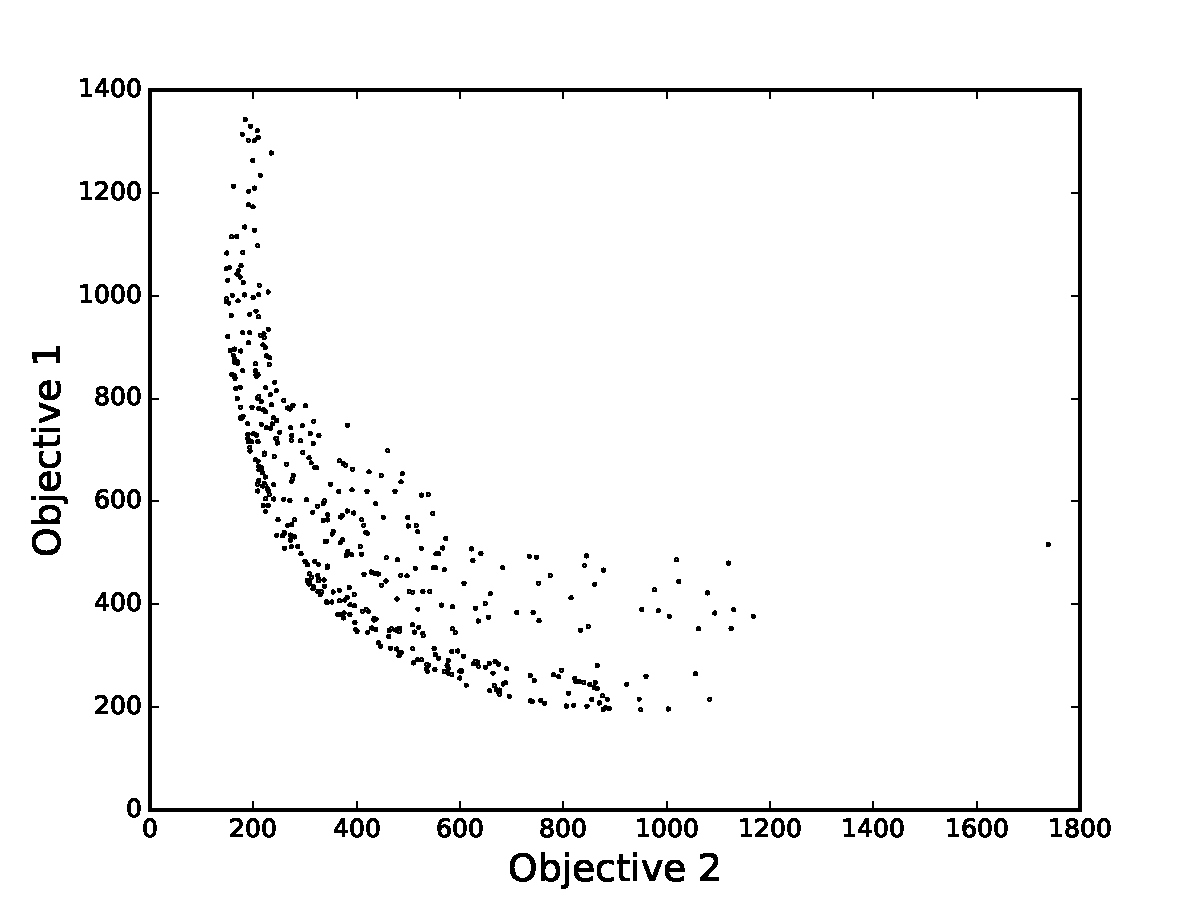
\includegraphics[width=\linewidth]{figures/TradeOffCurveFasterCooling}
       \caption{The black dots represent the rank 0, or best parameter sets, and the grey dots represent rank 1-4 parameter sets.}
       \label{fig:tradeoffcurve}
\end{figure}
\begin{figure}[ht]
       \centering
       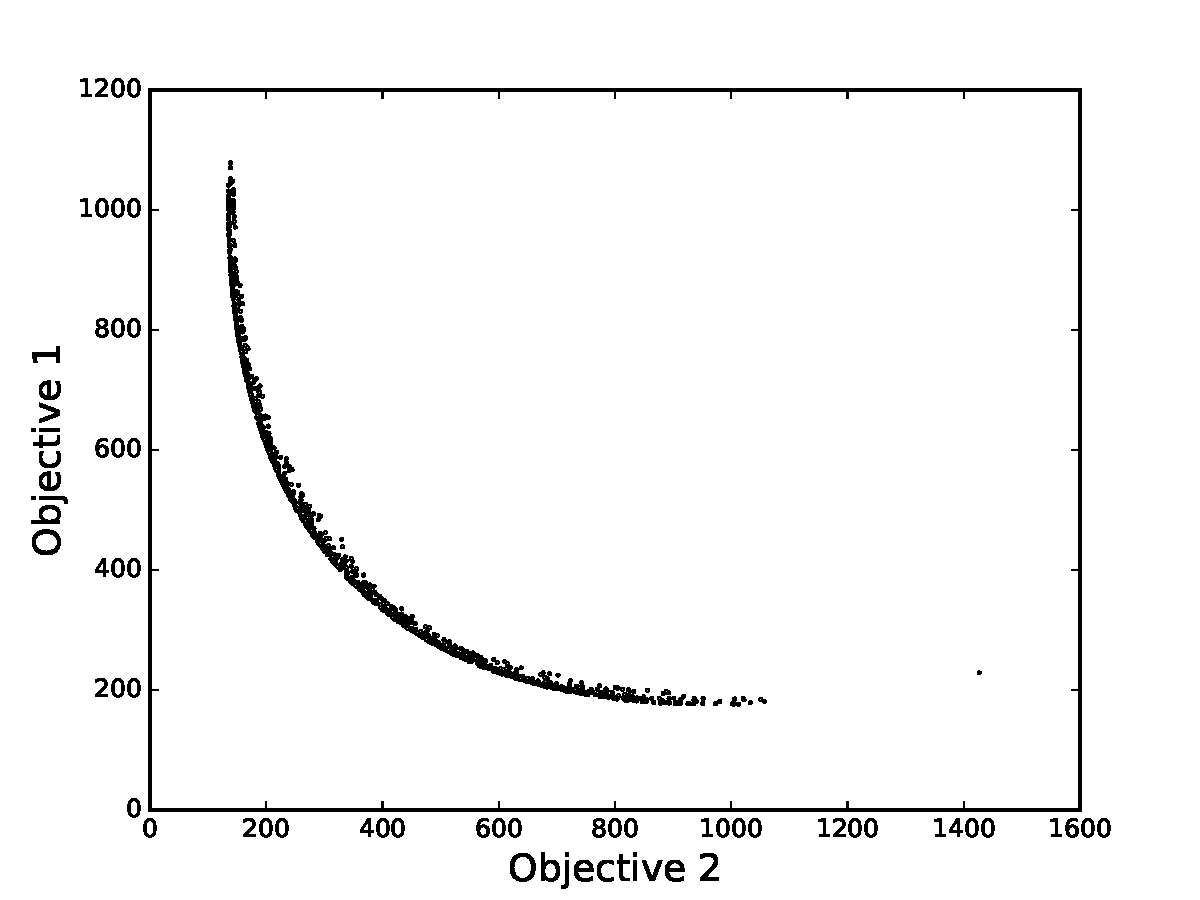
\includegraphics[width=\linewidth]{figures/TradeOffCurveSlowerCooling}
       \caption{The black dots represent the rank 0, or best parameter sets, and the grey dots represent rank 1-4 parameter sets.}
       \label{fig:tradeoffcurveslower}
\end{figure}


%\begin{table}[ht]
%\centering
%\caption{Original and estimated parameter values. The bolded parameters were held constant.}
%\label{tab:SingleParamsOptim}
%\begin{tabular}{|l|l|l|l|l|l|l|l|l|l|l|l|l|l|l|}
%\hline
%Parameter                                 & \textbf{$\alpha$} & $N$    & \textbf{$M$} & $k_1$ & \textbf{$k_2$} & $\tau_1$ & $\tau_2$ & $\tau_{ach}$ & $\tau_{nor}$ & \textbf{$\beta$} & $h_0$ & $m_{nor}$ & $m_{ach}$ & \textbf{$\tau_d$} \\ \hline
%Original Value                            & 1.5               & 75     & 120          & 1.5   & 0.5            & 0.5      & 250      & 0.5          & 0.5          & 6                & 1.67  & 0.96      & 0.7       & 7                 \\ \hline
%Parameter Estimations from MIMIC II  Data & 1.5               & 75.319 & 120          & 2.299 & 0.5            & 1.345    & 0.126    & 250.339      & 3.185        & 6                & 1.412 & 0.160     & 2.35E-06  & 7                 \\ \hline
%\end{tabular}
%\end{table}

\begin{table}[ht]
\centering
\scriptsize
\caption{Original and estimated parameter values. The bolded parameters were held constant.}
\label{tab:SingleParamsNLopt}
\begin{tabular}{|l|l|l|l|l|l|l|l|l|l|l|l|l|l|l|}
\hline
Parameter                                 & \textbf{$\alpha$} & $N$    & \textbf{$M$} & $k_1$  & \textbf{$k_2$} & $\tau_1$ & $\tau_2$ & $\tau_{ach}$ & $\tau_{nor}$ & \textbf{$\beta$} & $h_0$ & $m_{nor}$ & $m_{ach}$ & \textbf{$\tau_d$} \\ \hline
Original Value                            & \textbf{1.5}      & 75     & \textbf{120} & 1.5    & \textbf{0.5}   & 0.5      & 250      & 0.5          & 0.5          & \textbf{6}       & 1.67  & 0.96      & 0.7       & \textbf{7}        \\ \hline
Parameter Estimations from MIMIC II  Data & \textbf{1.5}      & 107.33 & \textbf{120} & 41.139 & \textbf{0.5}   & 14.062   & 202.925  & 2.94E-05     & 8.156        & \textbf{6}       & 1.474 & 0.165     & 5.20E-02  & \textbf{7}        \\ \hline
\end{tabular}
\end{table}

\begin{table}[]
\centering
\scriptsize
\caption{Average parameter values for the 10 best sets per cluster. Data is reported as mean $\pm$ stdev. Bolded columns were held constant.}
\label{tab:MultiobjectiveParams}
\begin{tabular}{|l|l|l|l|l|l|l|l|l|l|l|l|l|l|l|}
\hline
Cluster & \textbf{$\alpha$} & $N$          & \textbf{$M$} & $k_1$          & \textbf{$k_2$} & $\tau_1$       & $\tau_2$        & $\tau_{ach}$   & $\tau_{nor}$   & \textbf{$\beta$} & $h_0$           & $m_{nor}$      & $m_{ach}$       & \textbf{$\tau_d$} \\ \hline
1       & \textbf{1.5}      & $50.36\pm 9$ & \textbf{120} & $.9566 \pm .3$ & \textbf{0.5}   & $.1854\pm .13$ & $127.31 \pm 46$ & $.5968 \pm .4$ & $.3176\pm .06$ & \textbf{6}       & $1.245\pm .006$ & $.1816\pm .02$ & $.0434\pm .004$ & \textbf{7}        \\ \hline
2       & \textbf{1.5}      & $37.98\pm 9$ & \textbf{120} & $1.379\pm .7$  & \textbf{0.5}   & $.3621\pm .11$ & $82.88\pm 33$   & $.1410\pm .06$ & $.1688\pm.04$  & \textbf{6}       & $1.749\pm.05$   & $.1609\pm.02$  & $.0962\pm .06$  & \textbf{7}        \\ \hline
\end{tabular}
\end{table}


\begin{table}[h]
\centering
\caption{Average Overall State Sensitivity Coefficents For Single Objective Case}
\label{tab:OSSCsoriginalParams}
\begin{tabular}{|l|l|l|l|l|l|l|l|l|l|}
\hline
Parameter set        & $S_{N}$    & $S_{k_1}$ & $S_{\tau_1}$ & $S_{\tau_2}$ & $S_{\tau_{ach}}$ & $S_{\tau_{nor}}$ & $S_{h_0}$   & $S_{m_{ach}}$ & $S_{m_{nor}}$ \\ \hline
original parameters  &            &           &              &              &                  &                  &             &               &                \\ \hline
estimated parameters & $1.75\pm4$ & $.76\pm3$ & $.87\pm3$    & $.39\pm2$    & $0.31\pm1.8$     & $4.18\pm1.5$     & $19.9\pm 6$ & $6.69\pm2$    & $.76\pm 1.8$   \\ \hline
\end{tabular}
\end{table} 
%\begin{table}[]
%\centering
%\caption{Sensitivity by clusters}
%\label{tab:clusterSensitivity}
%\begin{tabular}{|l|l|l|l|l|l|l|l|l|l|}
%\hline
%Cluster   & $\frac{dh}{dN}$ & $\frac{dh}{k_1}$ & $\frac{dh}{\tau_1}$ & $\frac{dh}{tau_2}$ & $\frac{dh}{\tau_{ach}}$ & $\frac{dh}{\tau_{nor}}$ & $\frac{dh}{h0}$ & $\frac{dh}{m_{nor}}$ & $\frac{dh}{m_{ach}}$ \\ \hline
%Overall   & 4.8352          & 0.2500           & 0.5088              & 0.0033             & 0.0204                  & 0.5720                  & 19.9294         & 1.1339               & 4.4651               \\ \hline
%cluster 1 & 4.7152          & 0.2456           & 0.5027              & 0.0033             & 0.0201                  & 0.5755                  & 19.4780         & 1.1438               & 4.3593               \\ \hline
%cluster 2 & 4.9137          & 0.2528           & 0.5128              & 0.0033             & 0.0206                  & 0.5697                  & 20.2248         & 1.1275               & 4.5344               \\ \hline
%\end{tabular}
%\end{table}
\end{document}
              
            
